%% AMS Lessons Learned manuscript (AMS LaTeX Package V6.1).
%% Target journal: Artificial Intelligence for the Earth Systems (AIES), Lessons Learned.
%% Body limit 3000 words (excl. title page, abstract, references, captions, figures); <=3 figures.
%% Compile: latexmk -pdf main   (or pdflatex; bibtex; pdflatex; pdflatex)

\documentclass{ametsocV6.1}

\title{Hard conservation correctors can hide a degrading model during AI weather and climate training}

\authors{William E. Chapman,\aff{a}\correspondingauthor{William E. Chapman, wich6609@colorado.edu} John S. Schreck,\aff{b} and Yingkai Sha\aff{b}}

\affiliation{\aff{a}{Department of Atmospheric and Oceanic Sciences, University of Colorado Boulder, Boulder, Colorado}
\aff{b}{NSF National Center for Atmospheric Research, Boulder, Colorado}}

\abstract{AI weather and climate emulators increasingly incorporate physical principles into their formulation and training. One approach is to apply hard correctors that modify network outputs so that global mass, water, or energy budgets close exactly. Prior work introduced such training-time correctors in the CREDIT framework and reported reduced precipitation bias and improved stability. Motivated by those results, we fine-tuned a global atmosphere emulator with an active water-budget corrector, using the corrected prediction in the supervised loss and evaluating success through post-correction budget closure. By that measure, training appeared successful: every delivered field closed the moisture budget to machine precision. Beneath the correction, however, raw precipitation developed a growing global low bias over 12 epochs, while the required correction increased from about 2\% to roughly 24\%. The cause is a scale degeneracy: uniform scaling of raw precipitation is undone exactly by the inverse change in the correction factor, and is therefore invisible to a loss evaluated on the corrected output. This invariance removes the restoring force on raw precipitation amplitude, allowing other training pressures to drive drift. We recovered stable behavior by supervising the pre-correction prediction, penalizing its raw budget imbalance, and retaining the hard correction only for the delivered field. The required correction returned to less than 1\% within the next epoch. A controlled $2\times2$ ablation showed that the runaway occurred only when corrected-output supervision was combined with no imbalance penalty. The broader lesson is that exact closure after a hard correction verifies the corrector, not the underlying model. Training and evaluation should therefore monitor pre-correction predictions, raw budget residuals, and correction magnitudes whenever a corrector removes information from the supervised objective.}

\begin{document}

\maketitle

\section{Introduction}\label{sec:intro}

AI emulators of weather and climate are increasingly built to respect physical conservation laws rather than to approximate them, using hard correctors that rescale or project the network output so that global budgets of mass, water, and energy close exactly, applied at inference and, more recently, during training \citep{wattmeyer2025, sha2025, gregory2026floenet, chapman2025camulator}. Building on that line of work, we enabled a hard water-budget corrector during the fine tuning of a global emulator designed to simulate atmospheric variability from the time scale of days to centuries and obtained a model whose every delivered field closed the moisture budget to machine precision. The pre-correction precipitation beneath that correction was meanwhile drifting toward a large low bias, and the standard conservation diagnostic did not detect it. The constraint guaranteed exact budget closure while the underlying model degraded. This article describes how that happened, why the usual diagnostic missed it, and what to monitor instead.

Neural network emulators of weather and climate can match traditional numerical models on several deterministic forecast metrics \citep[e.g.,][]{bi2023,lam2023,kochkov2024} and increasingly target long, stable climate time-scale integrations \citep[e.g.,][]{bonev2023sfno, karlbauer2024healpix, wattmeyer2025, chapman2025camulator}, yet they do not inherit physical conservation laws by construction. A network can violate global mass, water, or energy budgets even when its pointwise error is small \citep{beucler2021,sha2025}. Soft constraints address this by adding the violation to the loss \citep{raissi2019physicsinformed,karniadakis2021physicsinformed,beucler2021}, whereas hard constraints project or rescale the output so that the constraint holds exactly \citep{beucler2021,zanetta2023,valente2025,harder2023hardconstrained,wattmeyer2025,sha2025}. The strategies can be combined: a soft penalty can shape the learned prediction while a hard correction guarantees closure of the delivered field \citep{beucler2021}.

Hard correctors are attractive because they guarantee closure to machine precision without tuning a penalty weight. In the CREDIT framework, mass and energy budgets are closed by correctors that adjust surface pressure and atmospheric energy after the network forward pass \citep{schreck2025,sha2025}, and a globally multiplicative precipitation corrector of the form introduced for the ACE models closes the water budget \citep{wattmeyer2023ace,wattmeyer2025}. Evaluating the supervised loss on the corrected output also appears reasonable: every training sample satisfies the intended budget, and prior studies show that conservation imposed during training can improve stability and precipitation behavior \citep{wattmeyer2025,sha2025}. We therefore expected that leaving the water corrector active during fine-tuning would make the learned model more physically faithful. Instead, the investigation traced a growing low bias in raw precipitation to a scale degeneracy, a non-identifiable direction of the training objective introduced by the correction.

\section{Data and Methods}\label{sec:methods}

\subsection{Emulator and training configuration}\label{sec:setup}

CAMulator \citep{chapman2025camulator} is a global atmospheric emulator trained to reproduce 6-hourly Community Atmosphere Model (CAM6) states on a $1.0^\circ$ grid with 32 hybrid sigma levels. Prognostic fields include winds, temperature, total specific humidity, surface pressure, and surface precipitation \citep[see][for full details]{chapman2025camulator}. Training minimizes a latitude- and variable-weighted error between the predicted and target next state. The experiments reported here come from a fine-tuning phase (a version~2 of the CAMulator model) in which the decoder blocks that emit every prognostic and diagnostic field, precipitation included, were trainable while the backbone was frozen; optimization used Adam at a fixed learning rate of $2.5\times10^{-5}$ with no weight decay.

\subsection{Global water-budget corrector}

The water corrector computes the globally integrated tendency of total column water, evaporation source, and precipitation sink. It then rescales predicted precipitation by the factor required to close the budget. We denote this factor $r$: $r=1$ means the raw prediction already closes, and the fractional correction is $r-1$. With evaporation and precipitation defined as positive source and sink magnitudes, respectively, the residual and sign convention are given in the appendix.

\subsection{Reference water budget from CAM6}

The target data themselves require almost no correction. Applying the same calculation to one year of CAM6 output (1459 6-hourly steps in 1980, after pairing consecutive states for the tendency) gives a mean correction of 0.024\% with a standard deviation of 2.22\%. The global precipitation sink balances evaporation at $1.72\times10^{10}$~kg~s$^{-1}$ (annual average) with near-zero mean storage. Persistent model corrections of order 10\% therefore do not originate in the target data. The 2.22\% per-step spread reflects the 6-hourly temporal discretization of the budget from time-averaged output, not a CAM6 conservation error.

\subsection{Training interventions and ablation design}\label{sec:fix}

With the reference budget established, we now describe the training configurations that produced the failure and its remedy. The baseline production configuration retained the hard water-budget corrector, evaluated supervised precipitation loss on the corrected output, and applied no raw-imbalance penalty.

After the required correction had grown to approximately 24\%, we resumed training from that checkpoint with two changes. First, the supervised loss was moved from the corrected output to the pre-correction prediction, restoring direct supervision of raw precipitation amplitude. Second, we added a soft penalty on the squared raw closure deviation, $(r-1)^2$, to encourage the network to reduce its own water-budget imbalance. The hard corrector remained active in the forward pass so that the delivered field continued to close the budget exactly (Fig.~\ref{fig:schematic}).

Because the production intervention changed both supervised-loss placement and the penalty simultaneously, we performed a controlled $2\times2$ ablation to separate their effects. Four short fine-tunes from a common checkpoint crossed the supervised target (corrected versus pre-correction prediction) with the penalty weight (0 versus 0.1). The ablation used a configuration that drifted faster than the production run, so its correction magnitudes are not directly comparable to the production trajectory in Fig.~\ref{fig:drift}a. We did not test inference-only correction because prior work found training-time conservation important for forecast stability \citep{sha2025}.

\subsection{Implementation and numerical precision}

Accumulating global reductions at bfloat16 precision corrupts the correction diagnostic: across 30 sampled steps, bfloat16 introduced correction errors averaging 0.22\% and reaching 0.52\%. This is a monitoring hazard rather than a cause of the failure, because the errors are roughly fifty to a hundred times smaller than the drift documented in Section~\ref{sec:results}\ref{sec:growth}. Float32 was adequate in our tests, and we used float64 to make numerical error negligible. The corrector must also return the raw imbalance explicitly so that it can be monitored and included in the loss rather than hidden inside an in-place operation.

\section{Results}\label{sec:results}

\subsection{Growth of the required correction and the raw precipitation bias}\label{sec:growth}

We first examine the original production configuration, in which the hard corrector was active during training, the supervised precipitation loss was evaluated on the corrected output, and no raw-imbalance penalty was applied. During fine-tuning the required correction grew from 2.4\% to 24.1\% over 12 epochs (Fig.~\ref{fig:drift}a, orange), while the delivered field continued to close the global water budget to machine precision at every step. The failure is insidious: the corrector rescaled predicted precipitation before the supervised error was evaluated, so the standard conservation diagnostic reported success throughout, and the deterioration surfaced only in quantities outside that pass-fail test. Over the same span the raw global precipitation error worsened from $-4.0\%$ to $-19.8\%$ of the CAM6 target, whereas the corrected error changed only from $-1.7\%$ to $-0.5\%$; the raw precipitation sink itself declined steadily toward a low plateau (Fig.~\ref{fig:drift}c). The model was still delivering an exactly conservative field, but only because the corrector was compensating for an increasingly biased raw prediction.

Four checks ruled out alternative sources of the drift. The same budget calculation applied to CAM6 showed near-zero mean imbalance, so the trajectory did not originate in the target data. A second training run in the same configuration reproduced the behavior and drifted further, with per-step corrections peaking above 60\%, ruling out a single anomalous optimization path. The mass and energy correctors remained near 0.01\% while the water correction grew (Fig.~\ref{fig:drift}d), indicating that the model had not simply become unstable in every conserved quantity. Finally, recomputing the global reductions at higher precision changed the correction by only tenths of a percent, far too little to explain a 24\% signal. Together, these checks pointed to the coupling between the precipitation corrector and the supervised loss.

The failure had two components, one in the model and one in the diagnostic. The raw precipitation amplitude developed a low bias, but the post-correction conservation metric could not reveal it because exact closure was guaranteed by construction. A growing correction alongside a nearly unchanged delivered field indicates that the corrector had removed information the supervised objective required to identify raw precipitation amplitude.

\subsection{Scale degeneracy in the corrected loss}\label{sec:mechanism}

A loss evaluated only on the corrected field carries no information about the raw global precipitation amplitude, because any uniform rescaling produces the same corrected output. The corrector rescales raw precipitation to whatever global total the budget demands: if the network doubled its entire precipitation field, the correction factor would halve and the delivered output would be unchanged.

Formally, let $P$ be the raw precipitation field, let $\mathbf{1}^{T}P$ denote its global total, with grid-cell area weights absorbed into the notation, and let $Q$ be the total precipitation required by the predicted storage tendency and evaporation. The correction operator $C$, corresponding to the water fixer in Fig.~\ref{fig:schematic} and defined in full in the appendix, preserves the normalized spatial pattern $P/(\mathbf{1}^{T}P)$ while replacing its global amplitude with $Q$:
\begin{equation}
C(P)
=
Q\frac{P}{\mathbf{1}^{T}P},
\qquad
C(\alpha P)
=
C(P),
\qquad
J_C(P)P
=
0,
\label{eq:null}
\end{equation}
for any positive scalar $\alpha$. The final equality follows because a perturbation along $P$ gives $P+\epsilon P=(1+\epsilon)P$, which is only a uniform rescaling and therefore leaves the corrected field unchanged. Thus, the raw-amplitude direction lies in the null space of the correction Jacobian, and a supervised loss evaluated only on $C(P)$ provides no restoring gradient along that direction.

We verified the invariance by uniformly rescaling CAM6 precipitation with $\alpha\in\{0.5,0.75,1.0,1.25,1.5\}$. The corrected field $C(\alpha P)$ was unchanged to machine precision, the correction factor scaled as $r\propto1/\alpha$, and the corrected-output loss remained flat, whereas the raw-output loss and imbalance penalty responded strongly. A finite-difference probe along $P$ likewise remained at roundoff, consistent with $J_C(P)P=0$. This test isolates precipitation scaling alone; during training, precipitation, evaporation, and storage change jointly.

The scale invariance explains why the corrected loss cannot restore raw amplitude, but not why the observed drift was consistently downward. We did not isolate that forcing. Plausible contributors include gradients from strongly supervised fields that share decoder weights with precipitation and the tendency of mean-squared-error training to favor under-prediction for displaced, heavy-tailed precipitation \citep{gilleland2009,subich2025}. Weight decay was disabled. The apparent plateau likely marks departure from uniform rescaling, which reintroduces opposing gradients through changes in the spatial pattern or other jointly predicted fields.

The contrast among correctors helps explain why the vulnerability became visible only for water. Mass and energy adjustments act on temperature, humidity, and surface pressure, which are supervised across many levels or through coupled terms. The water adjustment acts on precipitation, whose global amplitude became weakly identified after correction. Because the operators also have different null spaces, weak supervision alone is not a complete explanation. A null direction produces visible runaway only when it overlaps a degree of freedom that the remaining objective does not strongly constrain.

\subsection{Recovery under pre-correction supervision with a penalty}\label{sec:recovery}

Starting from the degenerate checkpoint, the stable configuration described in Section~\ref{sec:results}\ref{sec:fix}, with penalty weight 0.1, reduced the required correction from 24\% to below 1\% within one epoch and held it near zero for the next 64 epochs; over the final five epochs the mean correction was 0.4\% with a standard deviation of 0.9\%. Because the soft penalty targets $(r-1)^2$ directly, the collapse of the required correction is necessary but not sufficient evidence of an improved model. A partly independent indicator is the recovery of the raw precipitation sink toward the CAM6 reference (Fig.~\ref{fig:drift}c), which is independent only insofar as the supervised evaporation and storage tendency are unbiased. We did not measure raw-field forecast skill.

\subsection{Ablation of supervised target and penalty}\label{sec:ablation}

The controlled ablation isolated which change prevented the runaway and exposed its signature in the raw field. Crossing the supervised target with the imbalance-penalty weight produced a clean $2\times2$ interaction. Only the corrected-target cell without a penalty drifted: its required correction rose to 60--70\% within an epoch and then partially receded (Fig.~\ref{fig:ablation}a), a third independent occurrence of the runaway alongside the two production runs. The same cell shows the failure directly in the raw prediction, its global precipitation sink collapsing to roughly $1.0\times10^{10}$~kg~s$^{-1}$, some 40\% below the CAM6 reference, while the three stable cells hold near it (Fig.~\ref{fig:ablation}b). The two panels track one degradation from opposite sides: the growing correction the model demands, and the shrinking raw amplitude that correction compensates for.

The other three cells stayed centered near zero across four epochs with no systematic growth, at per-step means of 1.1\%, 0.5\%, and 0.1\% for pre-correction supervision without penalty, the penalty under corrected-target supervision, and the combined configuration, respectively. These are single runs, and the reported spreads (1.6--3.1\%) are within-run step-to-step variation rather than across-seed uncertainty, so the three stable cells are not distinguishable from one another at this sample size; the resolved contrast is the runaway cell against the other three. The runaway therefore requires the specific pairing of corrected-output supervision with no competing constraint, and restoring pre-correction supervision or adding the penalty each suppresses it on its own.

\section{Discussion and Conclusions}\label{sec:discussion}

\subsection{Generalization to other correction operators}\label{sec:lesson}

A hard corrector need not be excluded from every differentiable architecture \citep{beucler2021,zanetta2023,valente2025,harder2023hardconstrained}. The specific danger occurs when the corrected field is the sole supervised target and the correction operator has a nontrivial null direction corresponding to a physically meaningful property of the raw prediction. The loss then cannot identify that property unless another term constrains it.

This yields a general diagnostic beyond multiplicative precipitation correction. Let $C(\hat x)$ be a differentiable correction and let the supervised objective be $\mathcal{L}_{\mathrm{sup}}(x_{t+1},C(\hat x))$. Any perturbation $v$ satisfying $J_C(\hat x)v=0$ is locally invisible to that objective because
\begin{equation}
\left.\frac{d}{d\epsilon}\mathcal{L}_{\mathrm{sup}}\!\left(x_{t+1},C(\hat x+\epsilon v)\right)\right|_{\epsilon=0}
=\nabla_C\mathcal{L}_{\mathrm{sup}}^{T}J_C(\hat x)v=0.
\label{eq:generalnull}
\end{equation}
If $v$ represents a physically meaningful property and no other term identifies it, the raw model is nonidentifiable in that direction. The pretraining question is therefore not only whether the corrected field satisfies the constraint, but which information the correction removes from the learning problem.

For a multiplicative global rescaling, Eq.~\eqref{eq:null} shows that raw amplitude is invisible after correction, so during training that amplitude must be constrained independently. The configuration of Section~\ref{sec:results}\ref{sec:fix} does this by supervising the pre-correction prediction. Corrected-output supervision combined with a penalty also controls the degeneracy in our ablation (Section~\ref{sec:results}\ref{sec:ablation}), but that route stays tuning dependent through the penalty weight, whereas pre-correction supervision constrains amplitude directly.

The result applies most directly to deterministic rescalings and projections with null spaces that overlap weakly supervised model degrees of freedom, including global moisture, energy, mass, and surface-pressure fixers. It should not be generalized automatically to every constraint operator.

Evaluation must follow the same logic. A conservation diagnostic computed after a hard correction is fixed by construction and indicates only that the corrector was applied, so training and evaluation should separately track the pre-correction residual, the magnitude of the required correction, raw-field skill, and corrected-field skill. The correction factor is itself a model diagnostic: a growing correction can reveal deterioration even while the delivered field remains exactly conservative, which makes it the quantity to monitor during training and evaluation.

Why does raw drift matter if the corrected global mean remains accurate?
A large correction means that precipitation amplitude is increasingly set
by predicted evaporation and storage rather than by the raw precipitation
field itself. The corrector also adjusts only one global scalar, so it cannot
repair regional errors once the drift departs from uniform rescaling.
Finally, in free-running simulations the corrected state feeds back at every
step, and stability under large repeated corrections remains untested. The
concern is therefore lost diagnostic information and risk beyond the
correction null space, not demonstrated degradation of the corrected
product.

\subsection{Relation to prior work}\label{sec:prior}

Our result complements \citet{sha2025}, who report benefits from global conservation during training and inference, including reduced precipitation bias and improved long-range stability. Their work establishes that training-time conservation can help; ours identifies a coupling that can make it fail when the corrected output is the only supervised target.

The Ai2 Climate Emulator (ACE2) provides a close comparison \citep{wattmeyer2025}. Its corrector multiplies precipitation by a globally uniform factor to close the moisture budget (the same operator we analyze) and is applied before a mean-squared-error loss with no conservation penalty. ACE2 reports stable long integrations, with no drift in total atmospheric moisture and a realistic precipitation climatology. These diagnostics are computed after correction, however, and do not include the correction factor or the raw precipitation field. ACE2 therefore contains the same precipitation-amplitude null direction, but its published diagnostics do not establish whether training produced meaningful drift along that direction, which is exactly the post-correction blind spot we document. The comparison is at the level of diagnostics rather than a like-for-like stability test, since our measured drift is a per-training-step quantity whereas ACE2's reported stability is free-running and climatological. We do not claim that ACE2 exhibits the raw-amplitude degradation documented here.

\subsection{Limitations}\label{sec:limits}

The evidence comes from one emulator and one physical constraint. The stable production run changed both supervised-loss placement and penalty weight at once; the controlled $2\times2$ in Section~\ref{sec:results}\ref{sec:ablation} separates them and shows that either change alone prevents the runaway, but those four runs span only four epochs from a single checkpoint, so they establish the short-term dissociation rather than long-horizon behavior.

The reported correction is measured per teacher-forced training step, and we do not claim improved forecast skill or climate fidelity. The stable configuration remained near zero for 64 epochs, but longer free-running integrations are required to assess accumulated drift. The CAM6 reference is stationary across 1980--84, with annual mean corrections from 0.022\% to 0.029\% and standard deviations from 2.04\% to 2.29\%. Finally, any broader skill benefit rests on prior work rather than the experiments reported here, since we did not compare inference-only correction against training-time penalization.

%%%%%%%%%%%%%%%%%%%%%%%%%%%%%%%%%%%%%%%%%%%%%%%%%%%%%%%%%%%%%%%%%%%%%
% FIGURES
%%%%%%%%%%%%%%%%%%%%%%%%%%%%%%%%%%%%%%%%%%%%%%%%%%%%%%%%%%%%%%%%%%%%%

\begin{figure}[t]
\noindent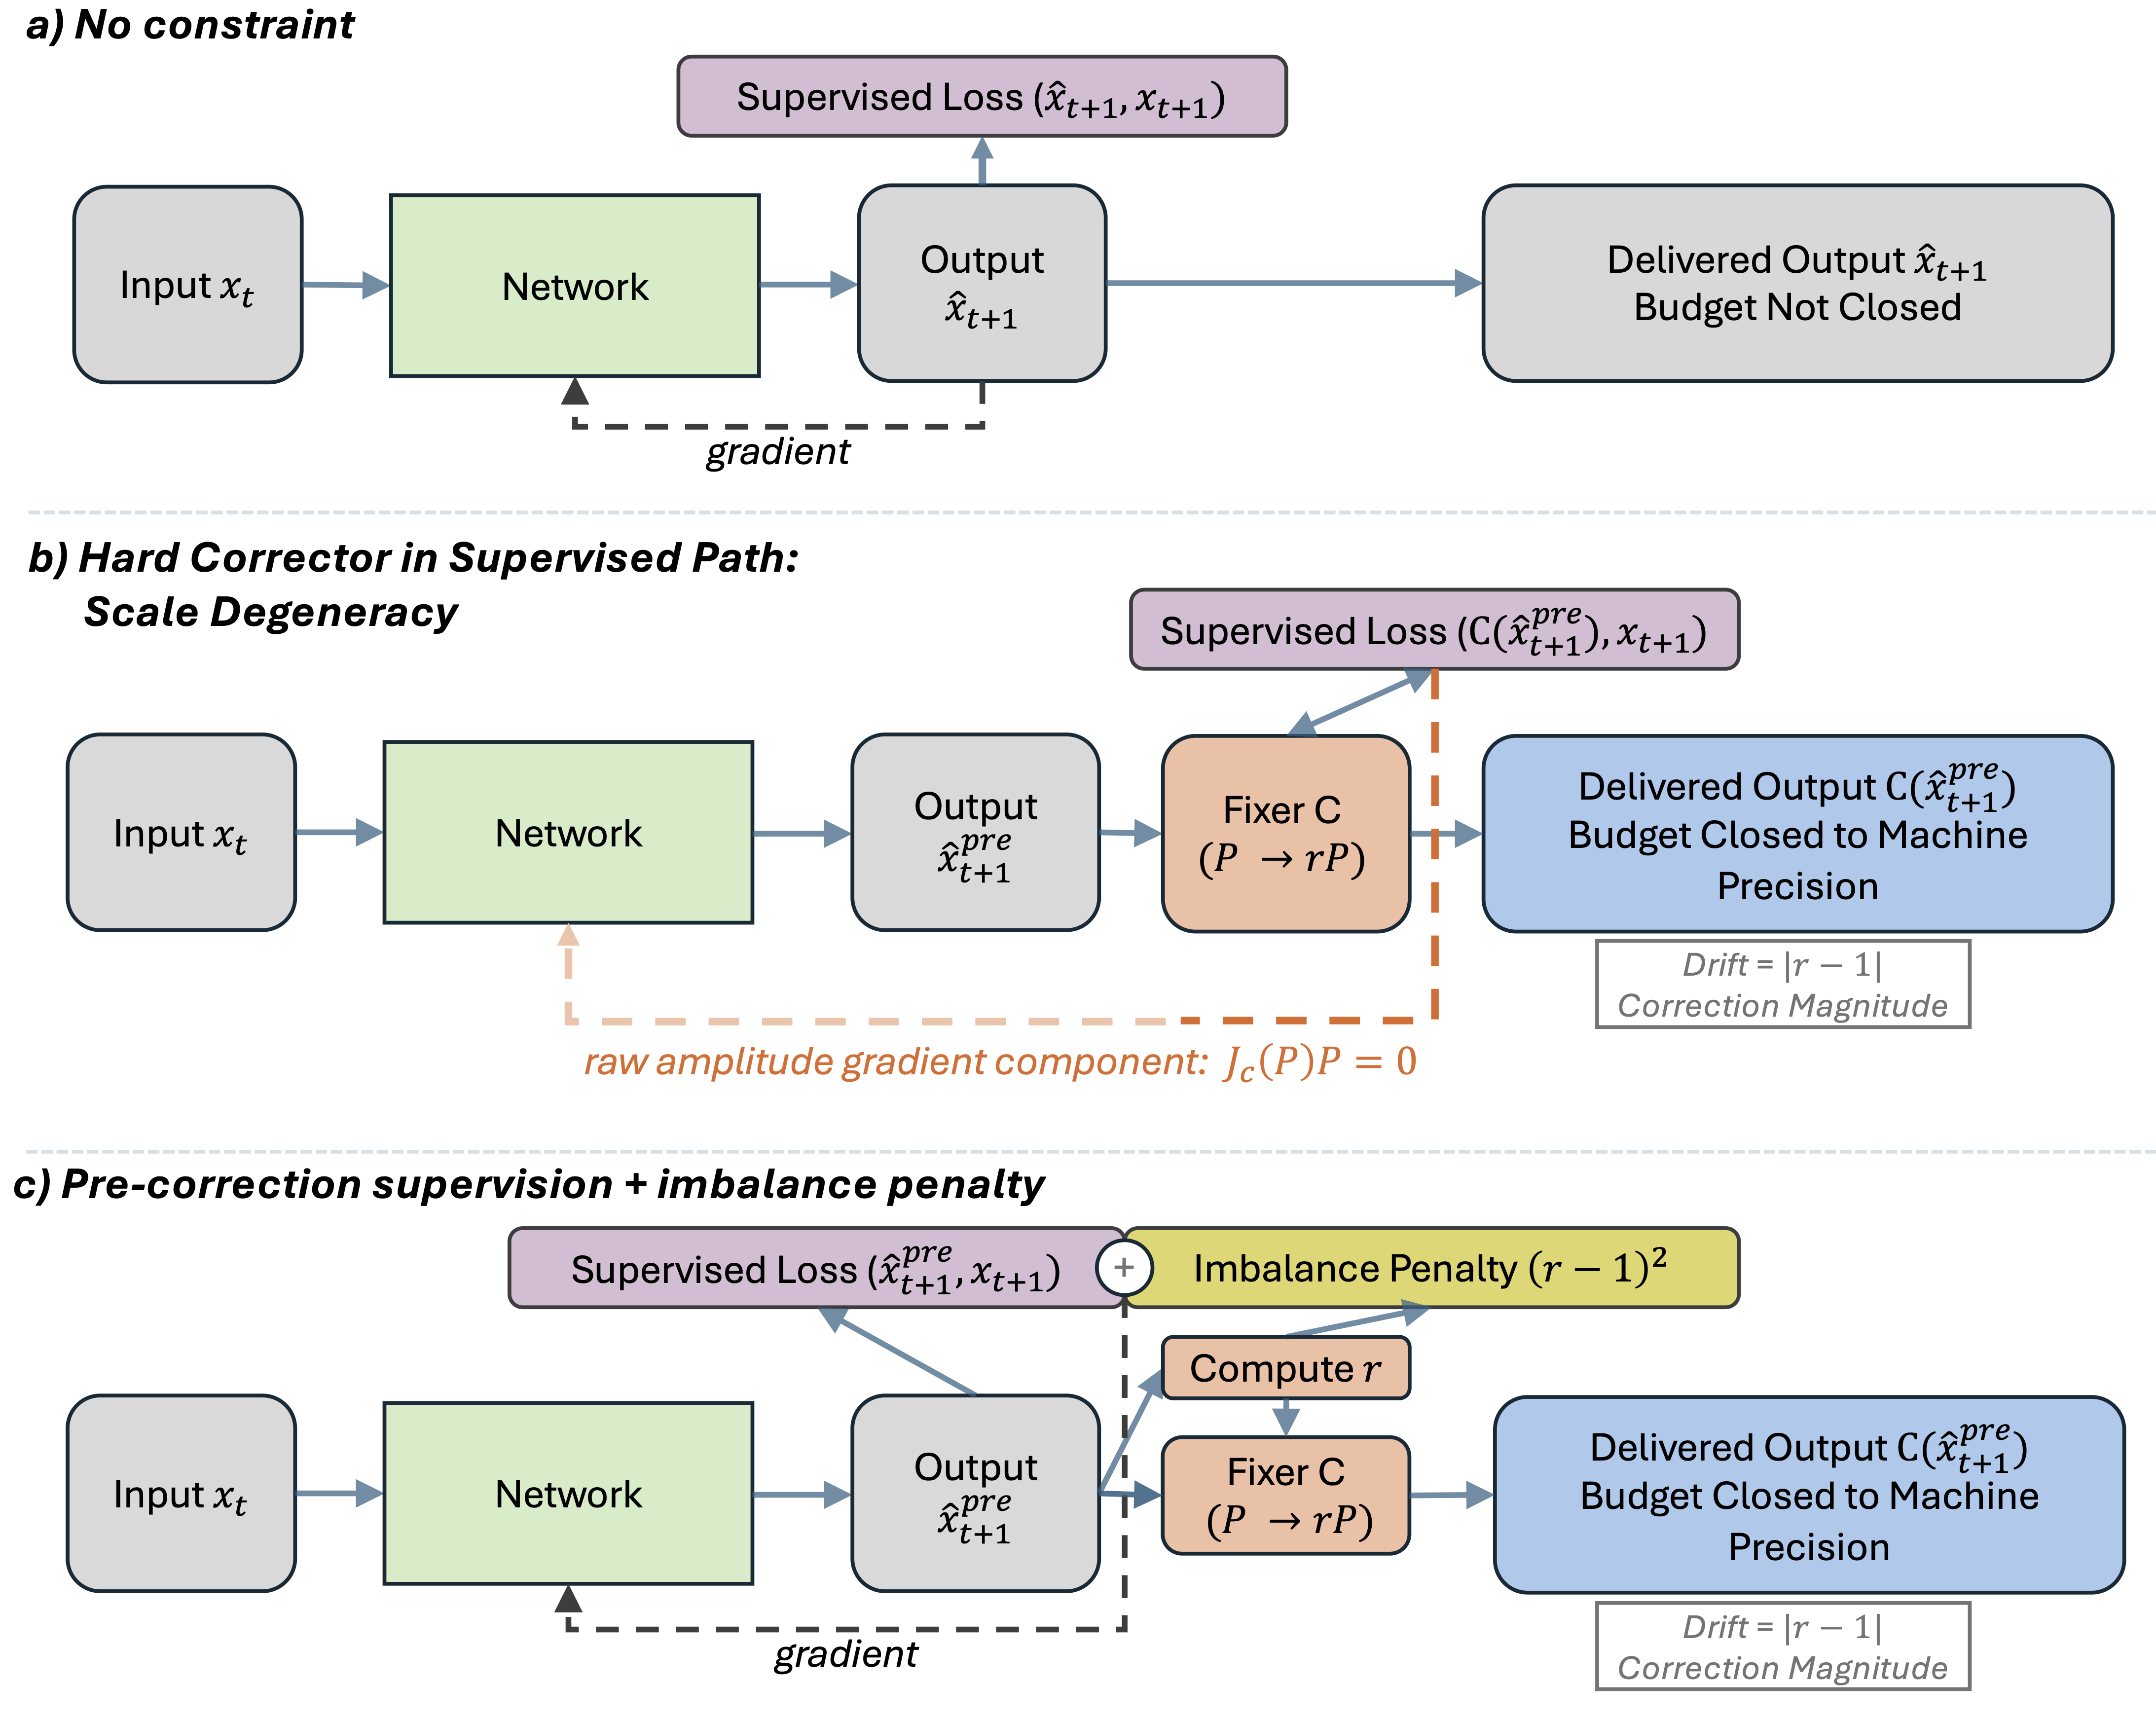
\includegraphics[width=35pc,angle=0]{fig01_schematic.png}\\
\caption{Training configurations for the water-budget corrector. The correction operator $C$ rescales the raw precipitation field $P$ by the budget-derived factor $r$, so that $P\rightarrow rP$ and the delivered field closes the global water budget exactly. (a)~Without a corrector, the supervised loss acts directly on the raw prediction and budget closure is not enforced. (b)~When the corrected prediction lies inside the supervised path, uniform scaling of $P$ is removed by the inverse change in $r$. The raw-amplitude gradient component therefore vanishes, $J_C(P)P=0$, even though the delivered field closes exactly. (c)~The supervised loss instead acts on the pre-correction prediction, while $r$ is computed from the raw budget and used both in the imbalance penalty $(r-1)^2$ and in the hard correction applied to the delivered field. Thus, raw amplitude and raw budget closure remain visible to the training objective while exact closure is retained at output.}
\label{fig:schematic}
\end{figure}

\begin{figure}[t]
\noindent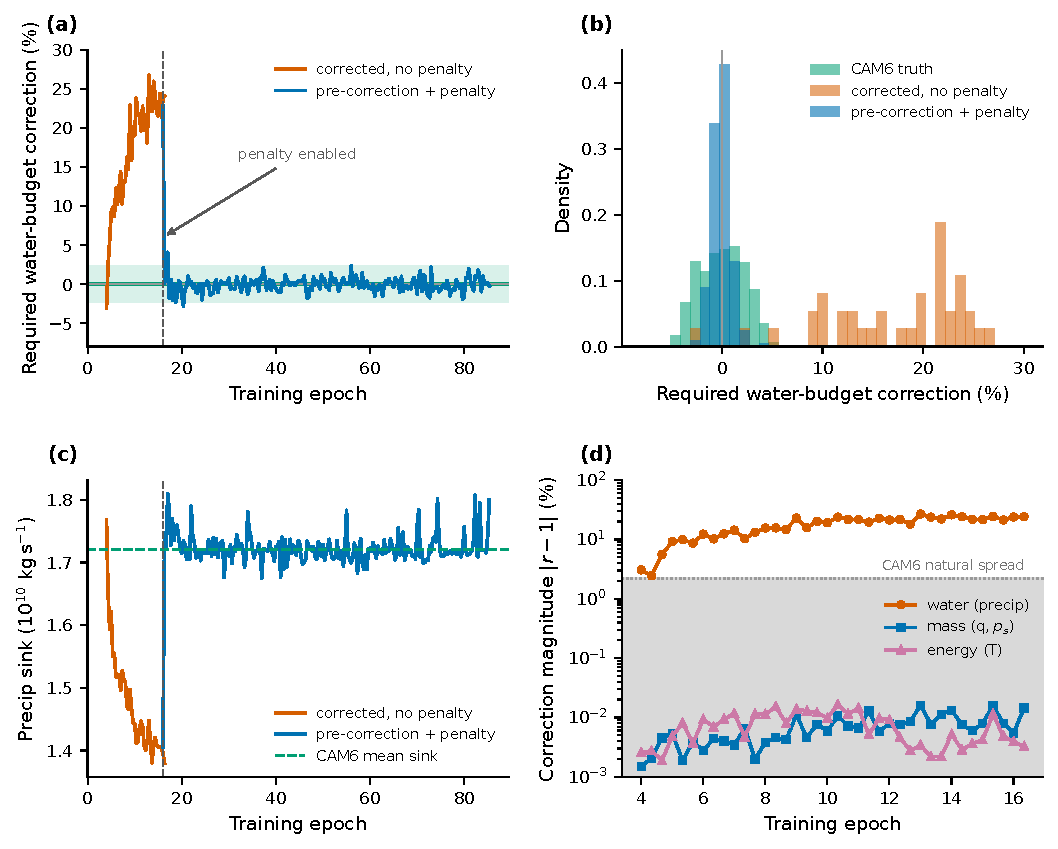
\includegraphics[width=33pc,angle=0]{fig02_finetune.pdf}\\
\caption{The corrected-output feedback during production fine-tuning and its recovery. (a)~In the corrected-output configuration, supervised loss is evaluated after correction and the required correction reaches about 24\% at the handoff (dashed line). After switching to pre-correction supervision with a penalty weight of 0.1, it returns to the CAM6 reference band (mean 0.024\%, $\pm$ one standard deviation 2.22\%). (b)~Correction distributions against CAM6; whenever the corrector is active the delivered field closes to machine precision, so the plotted quantity is the correction the raw model required. (c)~The raw global precipitation sink declines under corrected-output supervision and recovers under the combined formulation; the dashed line is the CAM6 annual-mean sink. (d)~Magnitudes of the global mass, water, and energy corrections ($|r-1|$, log scale) during the corrected-output run: water climbs from a few percent to about 24\%, whereas mass and energy remain within the CAM6 natural per-step spread (shaded). Mass and energy corrections act on strongly supervised prognostic fields, whereas the water correction acts on precipitation, whose global amplitude becomes weakly identified after correction.}\label{fig:drift}
\end{figure}

\begin{figure}[t]
\noindent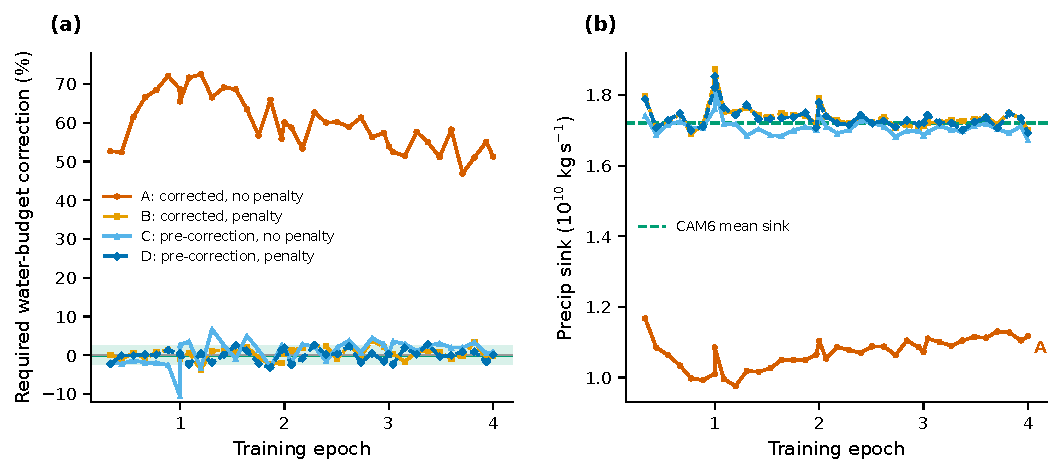
\includegraphics[width=33pc,angle=0]{fig03_ablation.pdf}\\
\caption{Controlled $2\times2$ ablation from a single checkpoint, crossing the supervised target (corrected, warm colors; versus pre-correction, cool colors) with the imbalance penalty weight (0 versus 0.1); one color and marker per cell. (a)~Required water-budget correction. Only cell A, corrected supervision with no penalty, runs away; supervising the pre-correction prediction (C) or adding the penalty (B) each holds drift near zero (CAM6 reference band shaded). The spreads are within-run step-to-step variation from single runs, so the three stable cells are not distinguished from one another. (b)~Raw global precipitation sink for the same four cells against the CAM6 mean sink (dashed): cell A's raw sink collapses to about $1.0\times10^{10}$~kg~s$^{-1}$ while the three stable cells hold near the reference, the physical consequence of the drift in~(a). The ablation uses a configuration that drifts faster than the production run, so its magnitudes are not directly comparable to Fig.~\ref{fig:drift}.}\label{fig:ablation}
\end{figure}

\clearpage

%%%%%%%%%%%%%%%%%%%%%%%%%%%%%%%%%%%%%%%%%%%%%%%%%%%%%%%%%%%%%%%%%%%%%
\acknowledgments
We acknowledge high-performance computing support from the Casper and Derecho (doi:10.5065/qx9a-pg09) systems provided by the Computational and Information Systems Laboratory (CISL) at the NSF National Center for Atmospheric Research (NCAR).

\datastatement
The model code, configurations, job scripts, and figure-generation code are available at \url{https://github.com/WillyChap/miles-credit/tree/camulator-conservation-lessons}, with the experiments organized under \texttt{experiments/}; the figures rebuild from cached data in \texttt{experiments/figure\_data/}. The CAM6 training data are Community Earth System Model output.

%%%%%%%%%%%%%%%%%%%%%%%%%%%%%%%%%%%%%%%%%%%%%%%%%%%%%%%%%%%%%%%%%%%%%
% APPENDIX
%%%%%%%%%%%%%%%%%%%%%%%%%%%%%%%%%%%%%%%%%%%%%%%%%%%%%%%%%%%%%%%%%%%%%
\appendix
\appendixtitle{The conservation-coupled training loss}

Let $x_t$ be the input state, $\hat x_{t+1}$ the network prediction of the next state, and $x_{t+1}$ the target next state. The supervised term is a latitude- and variable-weighted error,
\begin{equation}
\mathcal{L}_{\mathrm{sup}}(x_{t+1},\hat x_{t+1})=\frac{1}{V}\sum_{v=1}^{V}\frac{1}{BHW}\sum_{b,i,j}w_vL_i^{\mathrm{lat}}\ell\!\left(x_{b,v,ij},\hat x_{b,v,ij}\right),
\end{equation}
where $L_i^{\mathrm{lat}}=\cos(\varphi_i)^p/\overline{\cos(\varphi)^p}$ and $\ell$ is mean squared error.

For each sample $b$, the water corrector forms globally integrated total-column-water tendency, positive evaporation source, and positive precipitation sink,
\begin{equation}
\mathcal{T}_b=\!\sum_{ij}a_{ij}\frac{\mathrm{TWC}^{\mathrm{pred}}_{b,ij}-\mathrm{TWC}^{\mathrm{in}}_{b,ij}}{\Delta t},\quad
\mathcal{E}_b=\!\sum_{ij}a_{ij}\frac{E_{b,ij}\rho_w}{\Delta t},\quad
\mathcal{P}_b=\!\sum_{ij}a_{ij}\frac{P_{b,ij}\rho_w}{\Delta t}.
\end{equation}
Closure requires $\mathcal{T}_b=\mathcal{E}_b-\mathcal{P}_b$. The residual and precipitation correction factor are therefore
\begin{equation}
R_b=\mathcal{E}_b-\mathcal{T}_b-\mathcal{P}_b,\qquad
r_b=\frac{\mathcal{P}_b+R_b}{\mathcal{P}_b}=\frac{\mathcal{E}_b-\mathcal{T}_b}{\mathcal{P}_b},\qquad
r_b-1=\frac{R_b}{\mathcal{P}_b}.
\end{equation}
The corrector applies $P\!\to\!r_bP$. The soft penalty is the normalized raw imbalance,
\begin{equation}
\mathcal{L}_{\mathrm{water}}=\frac{1}{B}\sum_{b=1}^{B}(r_b-1)^2=\frac{1}{B}\sum_{b=1}^{B}\left(\frac{R_b}{\mathcal{P}_b}\right)^2.
\end{equation}
The stable objective is
\begin{equation}
\mathcal{L}=\mathcal{L}_{\mathrm{sup}}\!\left(x_{t+1},\hat x^{\mathrm{pre}}_{t+1}\right)+\lambda_w\mathcal{L}_{\mathrm{water}},
\label{eq:total}
\end{equation}
where $\hat x^{\mathrm{pre}}_{t+1}$ is the pre-correction prediction and $\lambda_w=0.1$ in the stable runs reported here. Evaluating the supervised term only on corrected precipitation removes the uniform-amplitude direction from that term, as shown by Eq.~\eqref{eq:null}; it does not by itself choose the direction of drift. Equation~\eqref{eq:total} restores direct supervision of raw amplitude and adds a gradient toward raw budget closure. Mass and energy correctors compute analogous factors but contribute no penalty here.

%%%%%%%%%%%%%%%%%%%%%%%%%%%%%%%%%%%%%%%%%%%%%%%%%%%%%%%%%%%%%%%%%%%%%
\bibliographystyle{ametsocV6}
\bibliography{references}

\end{document}
